\documentclass{uebblatt}

\newcommand{\sukk}{\mathrm{succ}}

\begin{document}

\maketitle{3}{\emph{Jedes Konzept ist eine Kan-Erweiterung.}}

\begin{aufgabe}{Limiten als Enden}
Sei~$F : \I \to \C$ ein Funktor. Zeige, dass ein Limes von~$F$ dasselbe ist wie ein
Ende von $\I^\op \times \I \to \I \stackrel{F}{\to} \C$. Als Formel: $\lim F =
\int_i F(i)$.
\end{aufgabe}

\begin{aufgabe}{Kan-Erweiterungen von darstellbaren Koprägarben}
Sei~$K : \M \to \C$ ein Funktor und~$X \in \M$. Zeige:
$\operatorname{Lan}_K \Hom_\M(X, \smallplaceholder) =
  \Hom_\C(K(X), \smallplaceholder)$.
\end{aufgabe}

\begin{aufgabe}{Die Limesformel für punktweise Kan-Erweiterungen}
Sei~$K : \M \to \C$ ein Funktor. Sei~$T : \M \to \A$ ein Funktor derart, dass
für alle Objekte~$c \in \C$ der Limes~$R(c) \defeq \lim_{f:c \to K(m)} T(m)$
existiert.
% Die Indexkategorie des Limes sieht also wie folgt aus:
% Objekte der Indexkategorie sind Morphismen c --> K(m), wobei m aus M beliebig
% sein kann.
% Morphismen zwischen c --> K(m) und c --> K(m') sind Morphismen g : m --> m'
% derart, dass das Dreieck mit den Kanten c --> K(m), K(g) und c --> K(m)
% kommutiert.
\begin{enumerate}
\item Erkläre, wie man diese Setzung zu einem Funktor~$R : \C \to \A$ ausdehnen
kann.
\item Beweise, dass~$R$ eine Rechts-Kan-Erweiterung von~$T$ längs~$K$ wird.
\end{enumerate}
\end{aufgabe}

\begin{aufgabe}{Kan-Erweiterungen längs volltreuer Funktoren}
Sei~$K : \M \to \C$ ein volltreuer Funktor. Sei~$T : \M \to \A$ ein Funktor
derart, dass die punktweise Links-Kan-Erweiterung~$\mathrm{Lan}_K(T)$
existiert. Zeige: Die kanonische natürliche Transformation~$T \Rightarrow
\mathrm{Lan}_K(T) \circ K$ ist ein Isomorphismus.
% Tipp: Die Kolimesformel für \mathrm{Lan}_K(T) lässt sich stark vereinfachen.
\end{aufgabe}

\begin{aufgabe}{Beispiele für transfinite Kompositionen in der Kategorie der Mengen}
\begin{enumerate}
\item Was ist die transfinite Komposition~$\NN \xra{\sukk} \NN \xra{\sukk} \NN
\xra{\sukk} \cdots$?
% Dabei ist succ : N --> N die Abbildung x |-> x + 1.
\item Sei~$f : X \to X$ eine Abbildung derart, dass sich für jedes~$x \in X$
die Folge~$(f^n(x))_{n \in \NN}$ stabilisiert. Was ist die transfinite
Komposition~$X \to X \to X \to \cdots$?
\item \emph{Für Fans von Garben.} Sei~$\F$ eine Garbe auf dem~$\RR^n$. Was ist
die transfinite Komposition der Einschränkungsabbildungen~$\F(B_1(0)) \to
\F(B_{1/2}(0)) \to \F(B_{1/3}(0)) \to \cdots$?
\end{enumerate}
\end{aufgabe}

{\centering
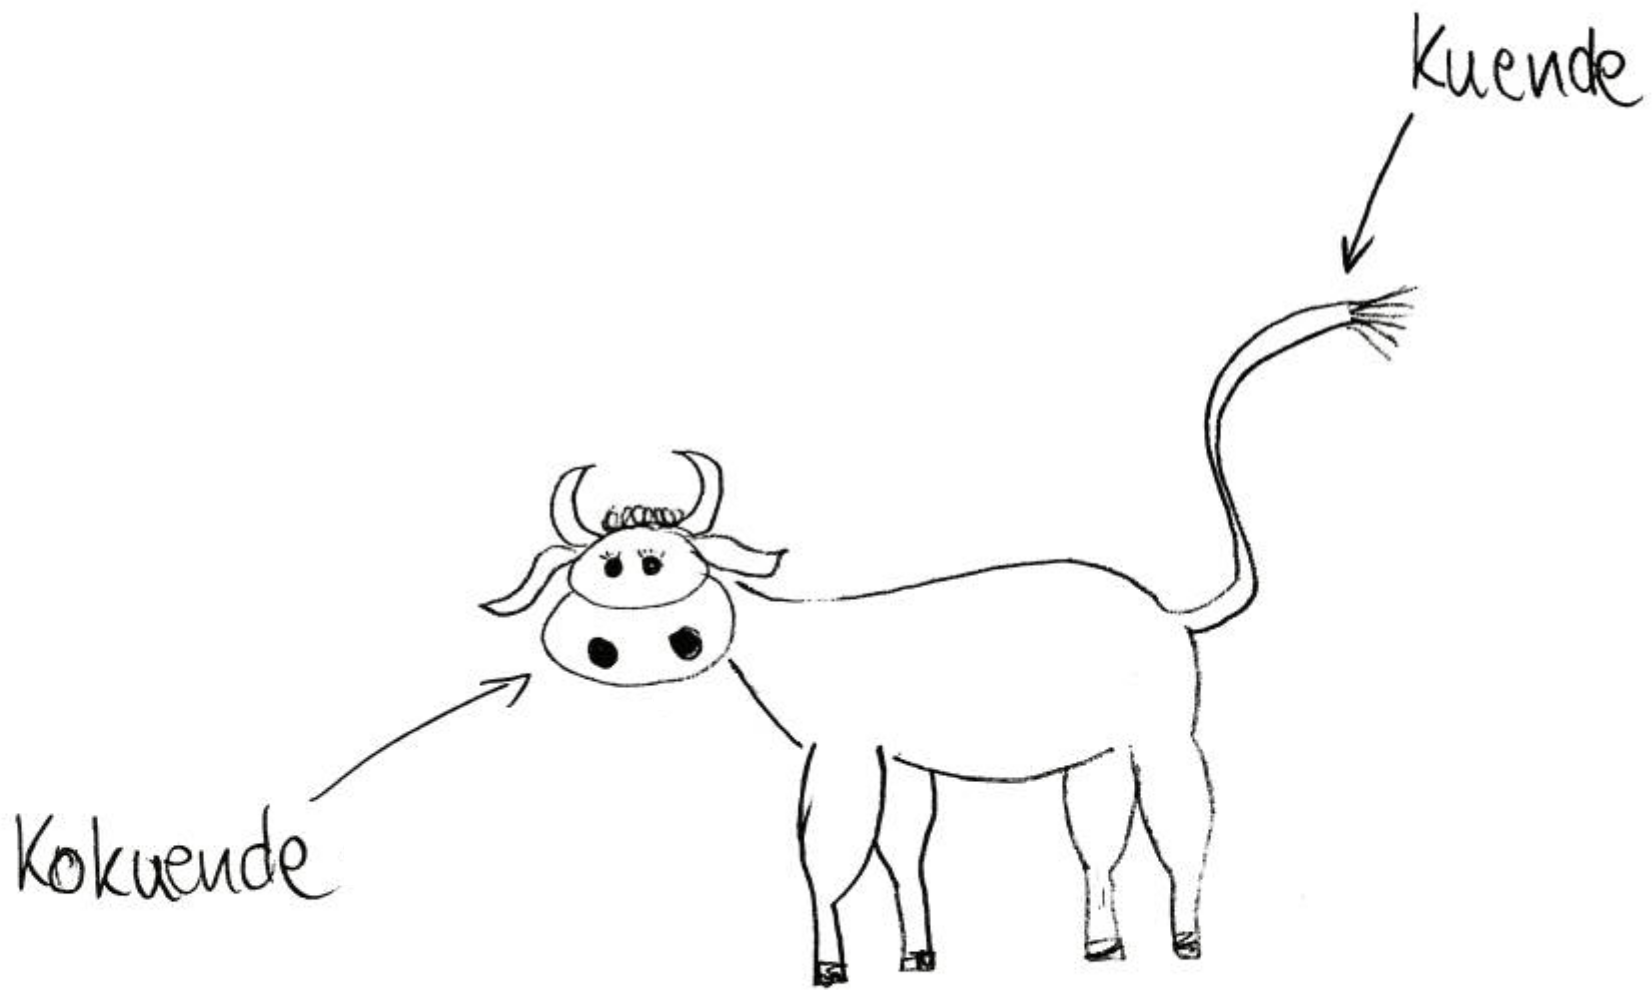
\includegraphics[scale=0.6]{images/kuende}
\par}
% mit besten Dank an Gesa

\newpage

\begin{aufgabe*}{Bonusaufgabe}{Bastelspaß in der Kategorie der topologischen Räume}
\begin{enumerate}
\item Was ist das Kofaserprodukt (Pushout) des folgenden Diagramms?
\[ \xymatrixcolsep{3pc}\xymatrixrowsep{3pc}\xymatrix{
  S^1 \ar[r] \ar@{^{(}->}[d] & \mathrm{pt} \ar@{-->}[d] \\
  D^2 \ar@{-->}[r] & ?
} \]
\item Überlege dir ein möglichst kniffliges Diagramm dieser Art und fordere
deine MitkohomologInnen heraus!
\end{enumerate}
\end{aufgabe*}

\end{document}

\begin{aufgabe}{Vertauschbarkeit von filtrierten Kolimiten mit endlichen Limiten}
Sei~$F : \C \times \D \to \Set$ ein Funktor.
\begin{enumerate}
\item Konstruiere einen kanonischen Morphismus~$\lambda : \colim\limits_{c \in \C}
\lim\limits_{d \in \D} F(c,d) \to \lim\limits_{d \in \D} \colim\limits_{c \in \C} F(c,d)$.
\item Sei~$\C$ sogar eine filtrierte Kategorie. Zeige, dass dann~$\lambda$ ein Isomorphismus ist.
\end{enumerate}
\end{aufgabe}

Kan-Erweiterungen als Adjungierte
